\documentclass[tikz,border=10pt]{standalone}
\usepackage{tikz}

\begin{document}
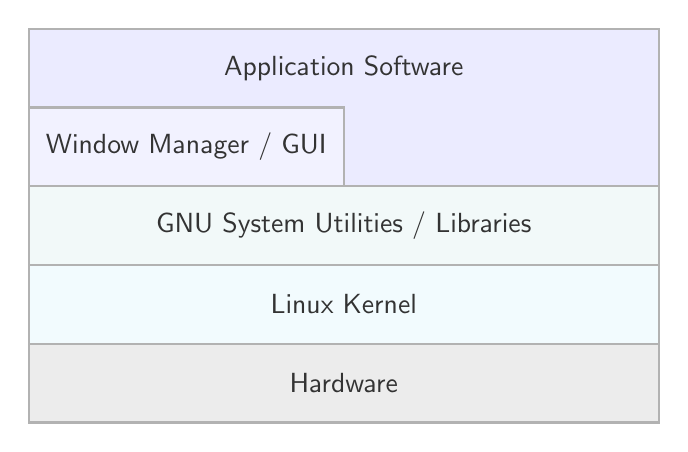
\begin{tikzpicture}[font=\sffamily, thick, align=center]
	% 1. 硬件层 (Hardware) - 基础灰
	\draw[fill=gray!15, draw=gray!60] (0, 0) rectangle (8, 1);
	\node[text=black!80] at (4, 0.5) {Hardware};

	% 2. 内核层 (Linux Kernel) - 淡雅水蓝
	\draw[fill=cyan!5, draw=gray!60] (0, 1) rectangle (8, 2);
	\node[text=black!80] at (4, 1.5) {Linux Kernel};

	% 3. 系统工具层 (GNU Utilities) - 浅灰青
	\draw[fill=teal!5, draw=gray!60] (0, 2) rectangle (8, 3);
	\node[text=black!80] at (4, 2.5) {GNU System Utilities / Libraries};

	% 4. 窗口管理器层 (Window Manager) - 静谧蓝
	\draw[fill=blue!5, draw=gray!60] (0, 3) rectangle (4, 4);
	\node[text=black!80] at (2, 3.5) {Window Manager / GUI};

	% 5. 应用软件层 (Application Software) - 略深浅蓝
	\draw[fill=blue!8, draw=gray!60] (0, 4) -- (0, 5) -- (8, 5) -- (8, 3) -- (4, 3) -- (4, 4) -- cycle;
	\node[text=black!80] at (4, 4.5) {Application Software};
\end{tikzpicture}
\end{document}